\section{Idee und Konzept}
Ich hatte schon immer den Traum, eines Tages mein eigenes Elektronikprodukt zu entwickeln, es zum Leben zu erwecken und bis zu einem kleinen kommerziellen Maßstab zu verkaufen.
Natürlich fand ich dabei besonderes Interesse im Bereich Smart Home sowie bei elektronischen Spielzeugen und Gadgets.
Hier kam mir ursprünglich die Idee eines würfelförmigen Spielzeugs, das aus einem Mikrocontroller und einem modernen \textcolor{blue}{OLED}-Display besteht, auf dem eine Art Tamagotchi dargestellt wird.
Dies ist natürlich ein Konzept, das bereits weit verbreitet ist und ohne erheblichen Marketingaufwand sowie besondere Alleinstellungsmerkmale kaum verkäuflich wäre.
\\\\
Trotz dieses Wissens wollte ich dennoch etwas Ähnliches umsetzen. So entstand die Idee des Smart-Home-Cubes \textbf{(SHC)}.
Kurz gesagt teilt er das gleiche äußere Erscheinungsbild, das ich mir für meine ursprüngliche Spielzeugidee vorgestellt hatte,
ist jedoch einfach ein Würfel, der mit allen erdenklichen Sensoren ausgestattet ist.
Alle diese Informationen sollen in Echtzeit übersichtlich auf dem \textcolor{blue}{OLED}-Frontdisplay dargestellt werden.
Zudem besteht die Möglichkeit zur Tasteninteraktion, um beispielsweise auf Abruf Mittelwerte von Temperatur oder Luftfeuchtigkeit anzuzeigen.
\\\\
Alle verschiedenen Sensoren sollen in Echtzeit ausgelesen und kontinuierlich ausgewertet werden.
Im Konzept sind sie alle an dieselbe \textcolor{blue}{I2C}-Busleitung angeschlossen.
Eine Übersicht aller Ziele ist unten dargestellt.
\subsection{Konzept Übersicht}
\begin{table}[h!]
\centering
\renewcommand{\arraystretch}{1.3}
\begin{tabularx}{\textwidth}{|l|X|X|}
\hline
\textbf{Kategorie} & \textbf{Ziel / Feature} & \textbf{Beschreibung} \\
\hline
\multirow{7}{*}{\textbf{Haupt Ziele}} 
    & Custom ESP32-S3 PCB Design      & Kern des Projektes \\
    & USB-C Support                   & Power + Data via USB-C \\
    & Feuchtigkeitssensor Sensor                 & Umgebungserfassung \\
    & Temperatur Sensor              & \\
    & Druck Sensor                 & \\
    & Strom Monitoring              & Stromverbrauch messung \\
    & Real-time OLED Display (1x)     & Echtzeitdarstellung der Messwerte \\
\hline
\multirow{7}{*}{\textbf{Optionale Ziele}}
    & 3D Case Design                  & 3D Gedruckt \\
    & 3× OLED Screens                 & Mehr Visuelles Feedback \\
    & Licht  Sensor                    & \\
    & UV Sensor                       & \\
    & CO\textsubscript{2} Sensor      & \\
    & Interaktive Sensor Interpretation & Dynamische, Steuerung(Knöpfe) \\
    & Daten speicherung \& Durchschnitt  & Historical statistics \\
\hline
\end{tabularx}
\caption{Übersicht der Haupt- und Nebenziele}
\end{table}
\newpage
\subsection{Visuelle Darstellung der Idee}
\begin{figure}[h]
    \centering
    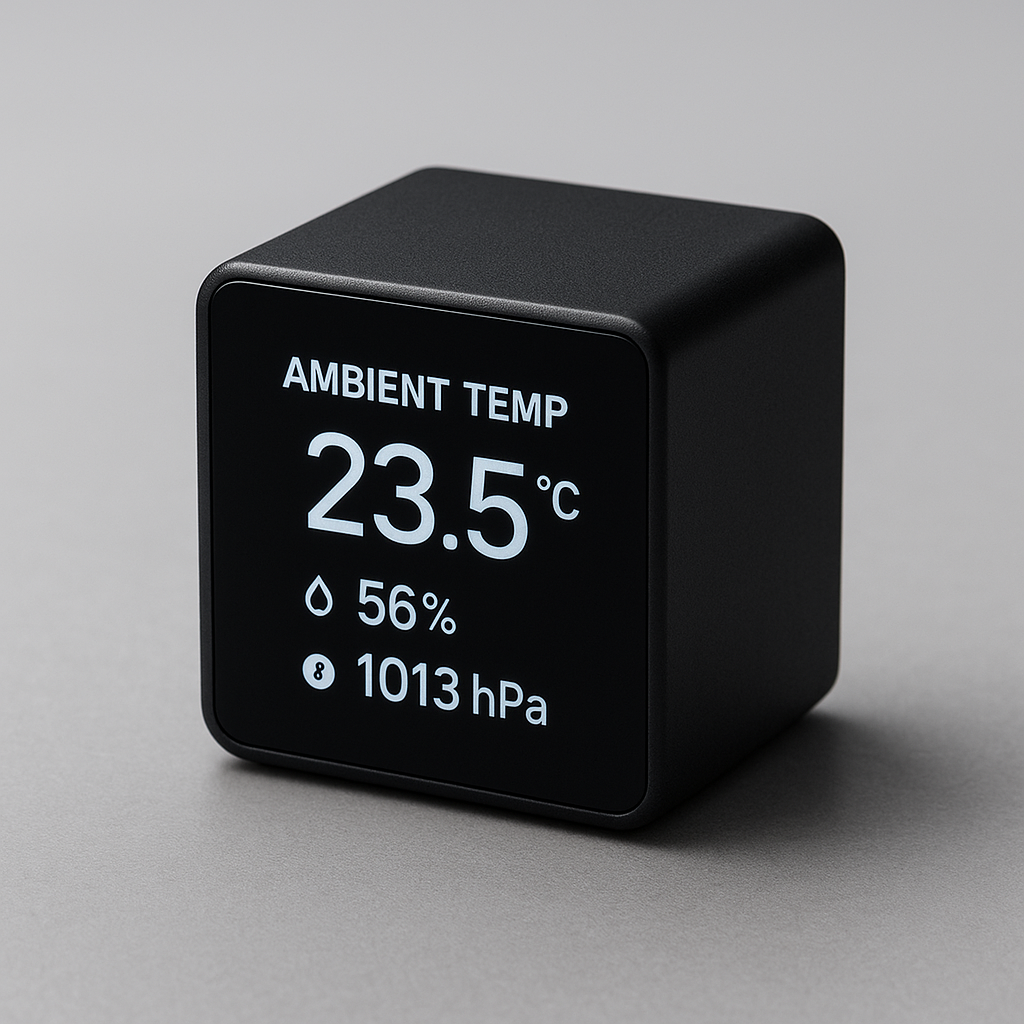
\includegraphics[width=1\linewidth]{images/cube.png}
    \caption{Concept Art\protect\footnotemark}
    \label{fig:v24}
\end{figure}
\footnotetext{Dieses bild wurde mithilfe von  OpenAI-GPT-5 generiert}
\newpage
\begin{figure}[h]
    \centering
    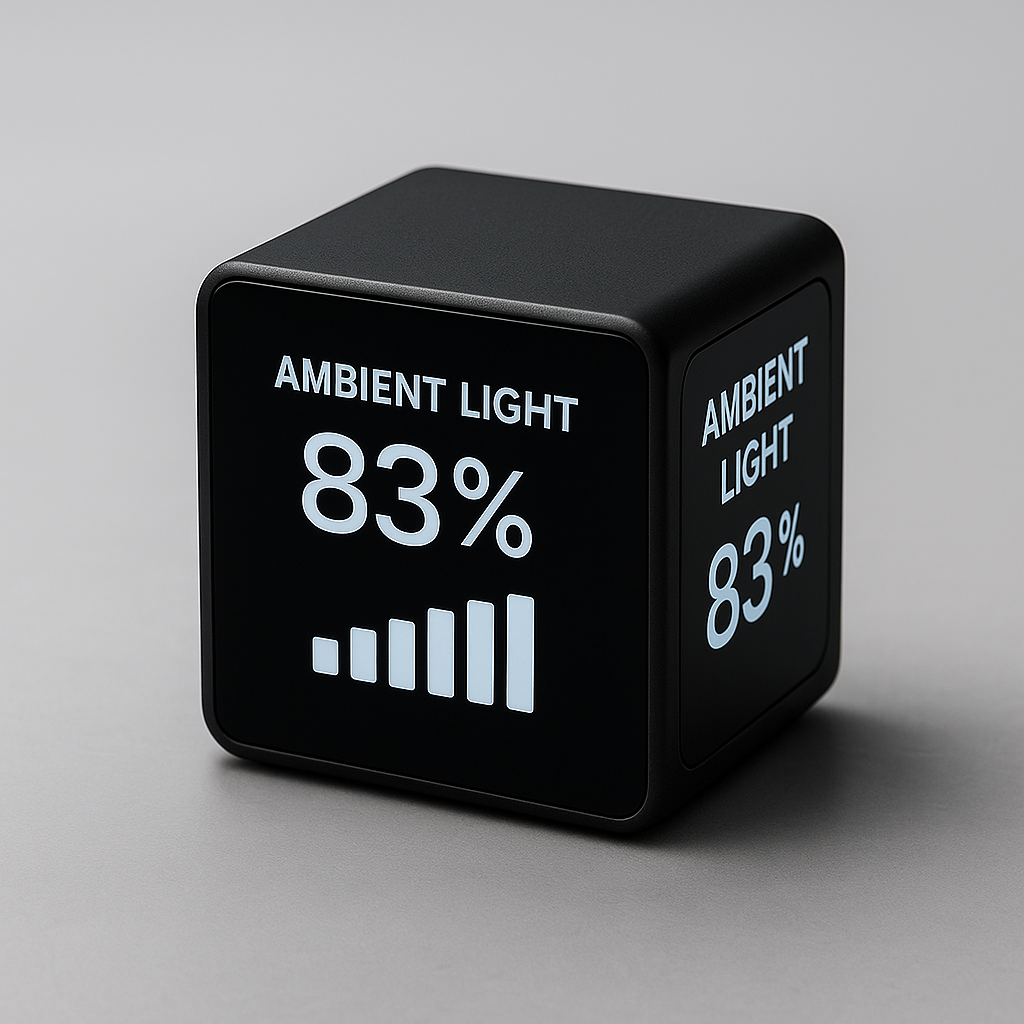
\includegraphics[width=1\linewidth]{images/cube2.png}
    \caption{Concept Art\protect\footnotemark}
    \label{fig:v24}
\end{figure}
\footnotetext{Dieses bild wurde mithilfe von  OpenAI-GPT-5 generiert}
\newpage
\begin{figure}[h]
    \centering
    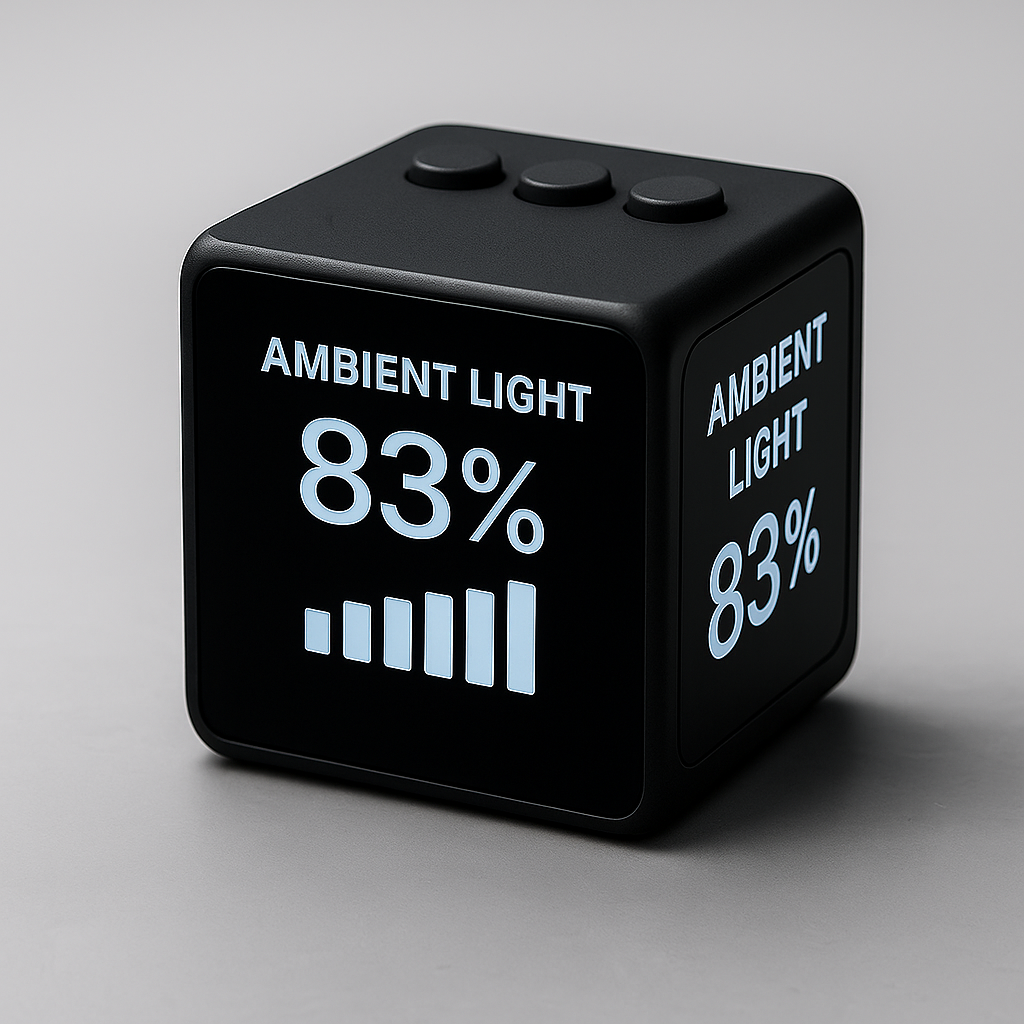
\includegraphics[width=1\linewidth]{images/cube3.png}
    \caption{Concept Art\protect\footnotemark}
    \label{fig:v24}
\end{figure}
\footnotetext{Dieses bild wurde mithilfe von  OpenAI-GPT-5 generiert}
\newpage
\begin{figure}[h]
    \centering
    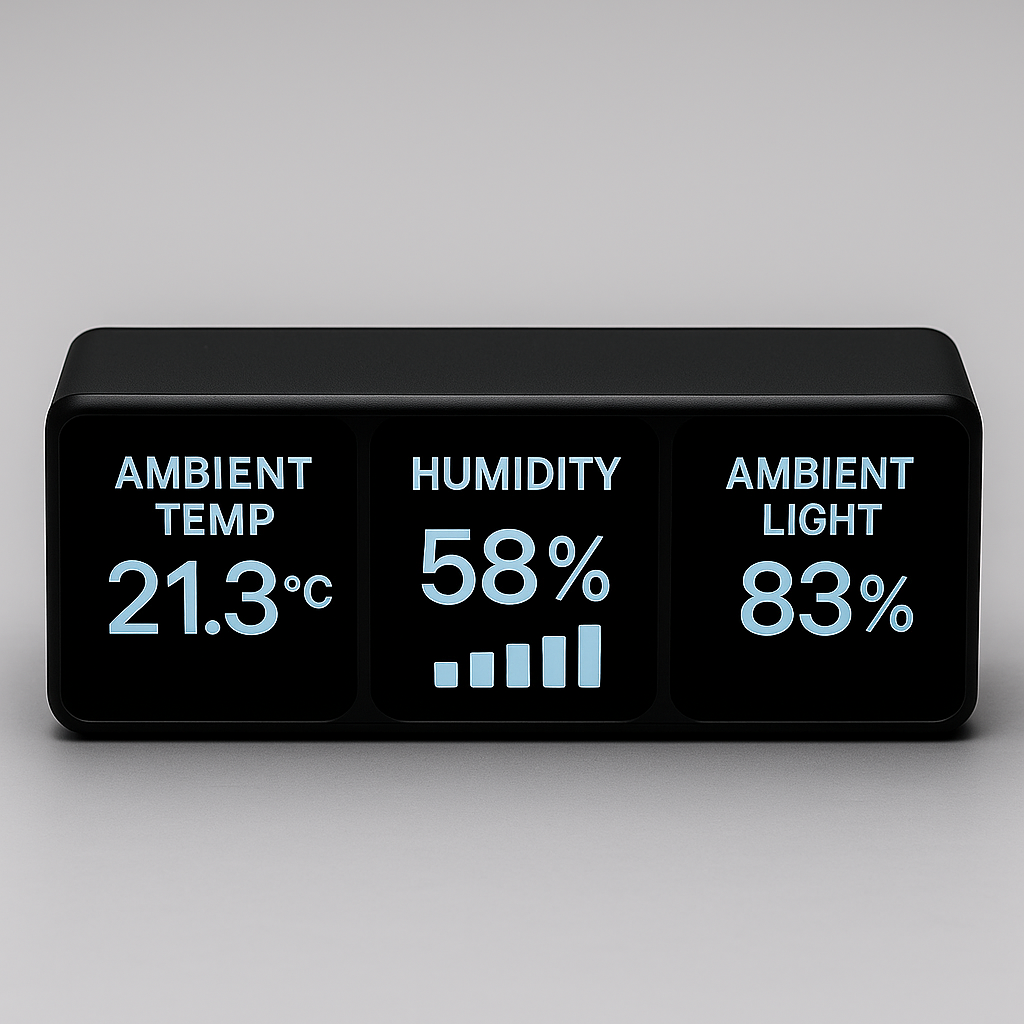
\includegraphics[width=1\linewidth]{images/cube4.png}
    \caption{Concept Art\protect\footnotemark}
    \label{fig:v24}
\end{figure}
\footnotetext{Dieses bild wurde mithilfe von  OpenAI-GPT-5 generiert}








